\documentclass{standalone}
\usepackage{tikz}

\begin{document}
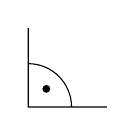
\begin{tikzpicture}
    % Draw the orthogonal lines
    %\draw[thick] (0, 0) -- (0, 2); % Vertical line
    %\draw[thick] (0, 0) -- (2, 0); % Horizontal line
    
    % from https://tex.stackexchange.com/questions/271229/how-can-i-make-a-right-angle-symbol-%E2%A6%9D
    \draw (0,1) -- (0,0) -- (1,0) (0.55,0) 
    % \draw (0,1) |- (1,0) (0.55,0)
	  arc(0:90:0.55);
    \fill (0.23,0.23) circle (0.05);

    % Place the symbol for the right ankle (R) in between
    % \node at (0.5, 0.5) {\textbf{R}};
\end{tikzpicture}
\end{document}
